%\pdfoutput=1
\documentclass[12pt,a4paper,reqno]{amsart}
\newcommand\hmmax{0}
\newcommand\bmmax{0}
\usepackage{amssymb}
\usepackage{amscd}
\usepackage[pdftex,pdfpagelabels]{hyperref}
\usepackage{enumerate}
\usepackage{comment}
%\usepackage{psfig}
\usepackage{graphicx}
\usepackage{cleveref}
\usepackage{siunitx}
\usepackage{tikz-cd}
\usepackage{stix}
\usepackage{bm}
\DeclareMathAlphabet\mathbfcal{LS2}{stixcal}{b}{n}
\numberwithin{equation}{section}

%\usepackage{mathabx}


\usepackage{mathtools}%                  http://www.ctan.org/pkg/mathtools
\usepackage[tableposition=top]{caption}% http://www.ctan.org/pkg/caption
\usepackage{booktabs,dcolumn}%           http://www.ctan.org/pkg/dcolumn + http://www.ctan.org/pkg/booktabs

% Lighter notation.
%\newcommand*\mc[1]{\multicolumn{1}{c}{#1}}
%\newcommand*\tupref[2]{\href{http://math.mit.edu/~primegaps/tuples/admissible_#1_#2.txt}{\num{#2}}}



%\DeclareMathOperator*\Kl{Kl} (commented because yield bad display for  \Kl_q %replaced with \newcommand... )
%\DeclareMathOperator*\FT{FT} (commented because yield bad display for \FT_q
%replaced with \newcommand...)

\DeclareMathOperator*\swan{swan}
\DeclareMathOperator*\cond{cond}
\DeclareMathOperator*\Gal{Gal}

\newcommand{\FT}{\mathrm{FT}}
\newcommand{\Kl}{\mathcal{K}\ell}
% Setup for ``caption''.
%\DeclareCaptionLabelSeparator{separation}{:\quad}
%\captionsetup{
  %font=small,
  %labelfont=sc,
  %labelsep=separation,
  %width=0.8\textwidth
%}

\DeclareFontFamily{OT1}{rsfs}{}
\DeclareFontShape{OT1}{rsfs}{n}{it}{<-> rsfs10}{}
\DeclareMathAlphabet{\mathscr}{OT1}{rsfs}{n}{it}

\addtolength{\textwidth}{3 truecm}
\addtolength{\textheight}{1 truecm}
\setlength{\voffset}{-.6 truecm}
\setlength{\hoffset}{-1.3 truecm}

\theoremstyle{plain}

\newtheorem{theorem}{Theorem}[section]
%\newtheorem{theorem}[theorem]{Theorem}
\newtheorem{proposition}[theorem]{Proposition}
\newtheorem{lemma}[theorem]{Lemma}
\newtheorem{corollary}[theorem]{Corollary}
\newtheorem{conjecture}[theorem]{Conjecture}
\newtheorem{heuristic}[theorem]{Heuristic}
\newtheorem{principle}[theorem]{Principle}
\newtheorem{question}[theorem]{Question}
\newtheorem{problem}[theorem]{Problem}
\newtheorem{claim}[theorem]{Claim}

\theoremstyle{definition}

%\newtheorem{roughdef}[subsection]{Rough Definition}
\newtheorem{definition}[theorem]{Definition}
\newtheorem{remark}[theorem]{Remark}
\newtheorem{remarks}[theorem]{Remarks}
\newtheorem{example}[theorem]{Example}
\newtheorem{examples}[theorem]{Examples}
%\newtheorem{problem}[subsection]{Problem}
%\newtheorem{question}[subsection]{Question}

\renewcommand\P{\mathbb{P}}
\newcommand\E{\mathbb{E}}
\newcommand\Var{\mathrm{Var}}
\newcommand\R{\mathbb{R}}
\newcommand\Z{\mathbb{Z}}
\newcommand\F{\mathbf{F}}
\newcommand\N{\mathbb{N}}
\newcommand\n{\mathbf{n}}
\renewcommand\a{\mathbf{a}}
\renewcommand\b{\mathbf{b}}
\renewcommand\j{\mathbf{j}}
\renewcommand\k{\mathbf{k}}
\renewcommand\v{\mathbf{v}}
\renewcommand\t{\mathbf{t}}
\renewcommand\r{\mathbf{r}}
\renewcommand\l{\mathbf{l}}
\newcommand\X{\mathbf{X}}
\newcommand\T{\mathbf{T}}
\newcommand\Y{\mathbf{Y}}
\newcommand\A{\mathbf{A}}
\newcommand\W{\mathbf{W}}
\newcommand\C{\mathbb{C}}
\newcommand\Q{\mathbb{Q}}
\renewcommand\Re{{\operatorname{Re}}}
\renewcommand\Im{{\operatorname{Im}}}
\newcommand\Log{{\operatorname{Log}}}
\newcommand\lcm{{\operatorname{lcm}}}
\renewcommand\gcd{{\operatorname{gcd}}}
\newcommand\eps{\varepsilon}
\newcommand\deriv{\zeta}
\newcommand\zero{\lambda}

\renewcommand{\mod}{\bmod}

\parindent 0mm
\parskip   5mm


\begin{document}

\title{Notes on upper and lower bounding $t(N)$}

\author{Terence Tao}
\maketitle

%%%%%%%%%%%%%%%%%%%%%%%%%%%%%%%%%%%%%%%%%%%%%%%%%

\section{Basics}

$t(N)$ denotes the largest quantity such that $N!$ can be factored into $N$ factors, each of which is at most $t(N)$.

$\nu_p(N)$ denotes the $p$-adic valuation of $N$, i.e., the exponent of the largest power of $p$ dividing $N$.

We recall Legendre's formula
\begin{equation}\label{legendre}
  \nu_p(N) = \sum_{j=1}^\infty \left\lfloor \frac{N}{p^j} \right\rfloor = \frac{N - s_p(N)}{p-1}.
\end{equation}

Asymptotically, it is known that
$$ \frac{1}{e} - \frac{O(1)}{\log N} \leq \frac{t(N)}{N} \leq \frac{1}{e} - \frac{c_0+o(1)}{\log N}$$
where
  \begin{align*}
    c_0 &\coloneqq \frac{1}{e} \int_0^1 \left \lfloor \frac{1}{x} \right\rfloor \log \left( ex \left \lceil \frac{1}{ex} \right\rceil \right)\ dx \\
    &= \frac{1}{e} \int_1^\infty \lfloor y \rfloor \log \frac{\lceil y/e \rceil}{y/e}\ \frac{dy}{y^2} \\
    &= 0.3044\dots
  \end{align*}

To bound the factorial, we have the explicit Stirling approximation \cite{robbins}
\begin{equation}\label{stirling}
  N \log N - N + \log \sqrt{2\pi N} + \frac{1}{12N+1} \leq \log N! \leq N \log N - N + \log \sqrt{2\pi N} + \frac{1}{12N},
\end{equation}
valid for all natural numbers $N$. 

To estimate the prime counting function, we have the following good asymptotics up to a large height.

  \begin{theorem}[Buthe's bounds]\cite{buthe}  For any $2 \leq x \leq 10^{19}$, we have
  $$ \mathrm{li}(x) - \frac{\sqrt{x}}{\log x}\left(1.95 + \frac{3.9}{\log x} + \frac{19.5}{\log^2 x}\right) \leq \pi(x) < \mathrm{li}(x)$$
  and
  $$ \mathrm{li}(x) - \frac{\sqrt{x}}{\log x} \leq \pi^*(x) < \mathrm{li}(x) + \frac{\sqrt{x}}{{\log x}}.$$
  \end{theorem}
  
  For $x > 10^{19}$ we have the bounds of Dusart \cite{dusart}.  One such bound is
  $$ |\psi(x) - x| \leq 59.18 \frac{x}{\log^4 x}.$$
  
  For $a_+,a_- \in [0,+\infty]$, we define the asymmetric norm $|x|_{a_+,a_-}$ of a real number $x$ by the formula
  $$ |x|_{a_+,a_-} \coloneqq \max(a_+ x, -a_- x),$$
thus this is $a_+ |x|$ when $x$ is positive and $a_- |x|$ when $x$ is negative.  This function is Lipschitz with constant $\max(a_+,a_-)$.

\section{Powers of 2 and 3}

For every natural number $B$, let $\delta_B$ denote the smallest gap in the set $\{ \{b \frac{\log 3}{\log 2}\}: 0 \leq b < B \} \cup \{1\}$, where $\{x\} \coloneqq x - \lfloor x\rfloor$ denotes the fractional part of $x$.  Clearly this quantity is nonincreasing in $B$. Numerical calculations show that
$$
 \delta_B \leq \frac{2.7}{B} \hbox{ for } 1 \leq B \leq 1900
$$
see \Cref{fig-log}. By the monotonicity of $\delta_B$, we thus have
\begin{equation}\label{delta-b}
 \delta_B \leq \frac{2.7}{\min(B, 1900)}
\end{equation}
for all $B \geq 1$.

\begin{figure}
  \centering
  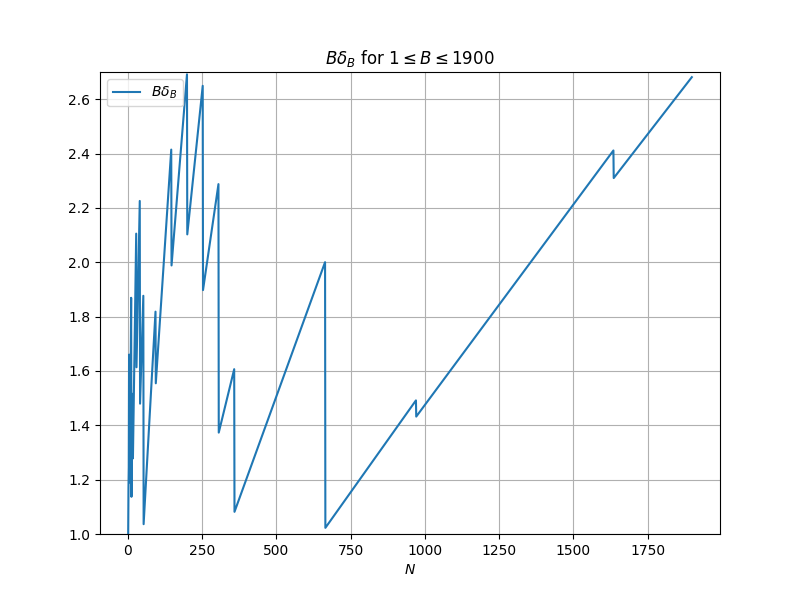
\includegraphics[width=0.8\textwidth]{log3_log2_plot.png}
  \caption{$B \delta_B$.}\label{fig-log}
\end{figure}

For larger values of $B$, $B \delta_B$ appears to be unbounded (presumably due to fluctuations in the continued fraction expansion of $\frac{\log 3}{\log 2}$).  However, one has the following decay bound.

\begin{proposition}  One has $\delta_B \ll B^{-c}$ for some absolute constant $c>0$.
\end{proposition}

\begin{proof} Let $N > 1$ be a parameter to be chosen later.  By Dirichlet's theorem, one can write $\frac{\log 3}{\log 2} = \frac{a}{q} + \frac{\eps}{q}$ for some $1 \leq q \leq N$ with $a,q$ coprime, and some $|\eps| \leq 1/N$.  From Baker's theorem we also have the lower bound $|\eps| \gg q^{-O(1)}$.  Writing $(mq+r) \frac{\log 3}{\log 2} = \frac{ar}{q} + (m+\frac{r}{q})\eps \hbox{ mod } 1$ for $r=0,\dots,q-1$ and $0 \leq m \leq \frac{1}{q\eps}$, we see that the gaps between these numbers on the unit circle do not exceed $O(1/N)$.  Since all of the $mq+r$ are of the size $O(N^{O(1)})$, we conclude that $\delta_B \ll 1/N$ for some $B = O(N^{O(1)})$, giving the claim.
\end{proof}

We can use these quantities to efficiently approximate a given number by a number of the form $2^m 3^n$.

\begin{lemma}  Let $t \geq 1$.  Then there exist natural numbers $n,m$ such that
  $$ t \leq 2^n 3^m \leq \exp( \delta_{\lceil \log t/\log 3 \rceil} \log 2 ) t.$$
In particular, if $N \leq 3^{1900} \approx 10^{906.5}$, one has
$$ t \leq 2^n 3^m \leq \exp( (2.7 \log 3 \log 2) / \log t ) t \leq \exp(2.06/\log t) t,$$
while for $t > 3^{1900}$, one has
$$ t \leq 2^n 3^m \leq t \exp( \frac{2.7 \log 2}{1900} )
\leq  \exp( 1/1000 ) t$$
and asymptotically one has
$$ t \leq 2^n 3^m \leq  \exp( O(\log^{-c} t) ) t$$
for some absolute constant $c>0$.
\end{lemma}

\begin{proof}  Set $B \coloneqq \lceil \log s/\log 3 \rceil$.  By definition of $\delta_B$, one can find $0 \leq m \leq B-1$ and an integer $n$ such that 
$$ \frac{\log s}{\log 2} \leq n + m \frac{\log 3}{\log 2} \leq \frac{\log s}{\log 2} + \delta_B.$$
Since $m \leq \log s/\log 3$, we see that $n$ must be non-negative.  Multiplying by $\log 2$ and exponentiating, we obtain the claim.
\end{proof}

\section{Criteria for lower bounding \texorpdfstring{$t(N)$}{t(N)}}

Suppose we are trying to factorize $N!$ into factors of size at least $t$.  A candidate tuple $\vec b = (b_1,\dots,b_{N'})$ is said to be \emph{admissible} if $b_j \geq t$ for all $j=1,\dots,N'$.  The \emph{$p$-saving} $S_p(\vec b)$ of the tuple is defined by the formula
$$ S_p(\vec b) \coloneqq \nu_p(N) - \sum_{i=1}^{N'} \nu_p(b_i).$$
A tuple is \emph{debt-free} if $S_p(\vec b) \geq 0$ for all $p$.

From the fundamental theorem of arithmetic we have
$$ \log b_i = \sum_p \nu_p(b_i) \log p$$
and 
$$ \log N! = \sum_p \nu_p(N!) \log p$$
and hence we obtain the identity 
\begin{equation}\label{ident}
   \log N! - \sum_{i=1}^{N'} \log b_i = \sum_p S_p(\vec b) \log p.
\end{equation}

By the fundamental theorem of arithmetic, we obtain a perfect factorization $N! = b_1 \dots b_{N'}$ if all the $p$-savings vanish.  The \emph{excess} $E(\vec b)$ is defined to be the quantity
\begin{equation}\label{excess} 
  E(\vec b) \coloneqq \sum_{i=1}^{N'} \log \frac{b_i}{t}.
\end{equation}
This quantity is non-negative for admissible tuples.  Intuitively, the smaller the excess, the more efficient the candidate factorization.  By combining \eqref{excess} with \eqref{ident} we obtain the identity
\begin{equation}\label{excess-save}
  E(\vec b) + \sum_p S_p(\vec b) \log p = \log N! - N' \log t.
\end{equation}

We conclude

\begin{proposition}  Let $2 \leq t \leq N$ with $t = N /e^{1+\delta}$.  Suppose one can find an admissible tuple $\vec b$ such that
\begin{equation}\label{main} 
  E(\vec b) + \sum_p |S_p(\vec b)|_{\log p,\infty}  \leq \delta N + \log \sqrt{2\pi N}.
\end{equation}
Then $t(N) \geq t$.
\end{proposition}

For the purposes of the Guy--Selfridge conjecture $t(N) \geq N/3$, we may take $\delta = \log \frac{3}{e} \approx 0.098$.  

In \cite[Proposition 3.1]{tao} the variant criterion
$$ 
E(\vec b)  + \sum_p |S_p(\vec b)|_{\log p,\log 2} + |N'-N| \log N \leq \delta N$$
was given in place of \eqref{main}, but the condition \eqref{main} seems slightly superior numerically (we no longer need to maintain direct control on $N'$).

\begin{proof}  From \eqref{main}, the tuple must be debt-free.  Applying \eqref{stirling}, we have
$$ E(\vec b) + \sum_p S_p(\vec b) \log p < \log N! - N\log t,$$
and hence by \eqref{excess-save} we have $N' \geq N$.
If we then delete all but $N$ of the terms in the tuple $(b_1,\dots,b_{N'})$, and then distribute all $p$-savings amongst these surviving terms arbitrarily, we obtain a factorization $N! = a_1 \dots a_N$ with all $a_i \geq t$, so that $t(N) \geq t$ as required.
\end{proof}

In view of this proposition, we no longer need to keep direct track of the number of terms in the factorization; as long as we keep the excess small, and have not too much $p$-saving, particularly at large primes, while staying debt-free, we get a lower bound on $t(N)$. 

For very large $N$, a promising strategy to improve the criterion is to initially allow for a large $2$-saving and $3$-saving, and then ``spend'' those available primes later on well chosen factors of the form $2^m 3^n$.  Here is a more precise formulation.

\begin{proposition}[Second criterion]  Let $2 \leq t \leq N$ with $t = N /e^{1+\delta}$.  Suppose we can find pairs $(m_1,n_1)$, $(m_2,n_2)$ of natural numbers with
\begin{equation}\label{atet}
   t \leq 2^{m_i} 3^{n_i} \leq e^\eps t \leq N
\end{equation}
for $i=1,2$ and some $\eps>0$.  Suppose we also have an admissible tuple $\vec b$ obeying the following axioms:
\begin{itemize}
  \item[(i)]  The vector
\begin{equation}\label{svec}
  (S^-_2(\vec b), S^-_3(\vec b))
\end{equation}
in $\R^2$ is a non-negative linear combination of $(m_1,n_1)$ and $(m_2,n_2)$.
  \item[(ii)]  We have
  \begin{equation}\label{main-2}
    \begin{split} 
&    E(\vec b) + \sum_{p>3} |S_p(\vec b)|_{\log p,\infty} \\
& \quad + \frac{3}{2} \log N + \frac{\eps \log 12}{2} \frac{N}{\log t} \leq \delta N + \log \sqrt{2\pi}.
    \end{split}
  \end{equation}
\end{itemize}
Then $t(N) \geq t$.
\end{proposition}

In practice, the $\frac{3}{2} \log N$ term is negligible. The point here is that this version of the criterion largely frees up the need to track the undershoot at $2$ and $3$, other than to verify the (quite mild) condition (i).  The quantity $\eps$ can be easily bounded by $\log 2$ in most cases, but one expects (based on the irrationality of $\log 3/\log 2$) that one can do better than this; and this quantity can be bounded numerically quite easily even for rather large $N$.

\begin{proof}  By hypothesis, the vector \eqref{svec} can be written as $s_1 (m_1,n_1) + s_2 (m_2,n_2)$ for some positive reals $s_1,s_2$.  Splitting into integer and fractional parts, we can thus write \eqref{svec} as the sum of $\lfloor s_1 \rfloor$ copies of $(m_1,n_1)$, $\lfloor s_2 \rfloor$ copies of $(m_2,n_2)$, and a vector with coefficients at most $(m_1+m_2, n_1+n_2)$.  If we then add $s_1$ copies of $2^{m_1} 3^{n_1}$ and $s_2$ copies of  $2^{m_2} 3^{n_2}$ to the admissible tuple, then it remains admissible and debt-free; but now $S_2(\vec b)$, $S_3(\vec b)$ are reduced to at most $m_1+m_2$, $n_1+n_2$ respectively.  Also, each $2^{m_i} 3^{n_i}$ contributes an excess of at most $\eps$, which in turn is at most $\frac{\eps}{\log t} \log 2^{m_i} 3^{n_i}$; hence the total additional excess produced here is at most $\frac{\eps}{\log t} \log 2^{S_2(\vec b)} 3^{S_3(\vec b)}$.  From \eqref{legendre} we have $S_p(\vec b) \leq \frac{N}{p-1}$, hence the additional excess is at most
$$ \frac{\eps}{\log t} \log 2^{N} 3^{N/2} \leq \frac{\eps \log 12}{2} \frac{N}{\log t}.$$
The new value of $S_2(\vec b) \log 2 + S_3(\vec b) \log 3$
is at most
\begin{align*}
  (m_1+m_2) \log 2 + (n_1+n_2)\log 3 &= \log 2^{m_1} 3^{n_1} + \log 2^{m_2} 3^{n_2} \\
  &\leq 2 \log N
  &= \frac{3}{2} \log N + \log \sqrt{N}.
\end{align*}
From \eqref{main-2} we conclude that the new admissible tuple obeys \eqref{main}, and the claim now follows from the previous proposition.  
\end{proof}

We can now allow for some debt at various primes $p$, as well as handle savings at small primes more efficiently.

\begin{proposition}[Third criterion]  Let $2 \leq t \leq N$ with $t = N /e^{1+\delta}$.  Suppose we can find pairs $(m_1,n_1)$, $(m_2,n_2)$ of natural numbers obeying \eqref{test}, and an admissible tuple $\vec b$ obeying the following axioms:
  \begin{itemize}
    \item[(i)]  The vector
  \begin{equation}\label{svec-2}
    (S_2(\vec b)-u, S_3(\vec b))
  \end{equation}
  in $\R^2$ is a non-negative linear combination of $(m_1,n_1)$ and $(m_2,n_2)$, whenever
  $$ 0 \leq u \leq \sum_{3 < p \leq \sqrt{t}} |S_p(\vec b)|_{\frac{2 \log p \lceil (\log t)/2\log 2 \rceil}{\log t}, \lceil \frac{\log p}{\log 2} \rceil} + \sum_{p>\sqrt{t}} |S_p(\vec b)|_{0,\lceil \frac{\log p}{\log 2} \rceil} + \left\lceil \frac{\log t}{\log 2} \right\rceil.$$
    \item[(ii)]  We have
    \begin{equation}\label{main-3}
      \begin{split} 
  &    E(\vec b) + \sum_{3 < p \leq \sqrt{t}} |S_p(\vec b)|_{\frac{2(\log p) \log 2}{\log t}, \log 2} + \sum_{p>\sqrt{t}} |S_p(\vec b)|_{\log p,\log 2} \\
  & \quad + \frac{3}{2} \log N + \frac{\eps \log 12}{2} \frac{N}{\log t} \leq \delta N.
      \end{split}
    \end{equation}
  \end{itemize}
  Then $t(N) \geq t$.
  \end{proposition}
  
The point here is that the ``cost'' of excessive savings at primes $3 < p \leq \sqrt{t}$ has been significantly reduced.  The condition (i) has become more complicated, but is easy to satisfy in practice.

\begin{proof} Suppose we have a $p$-debt $S_p(\vec b) < 0$ at some some prime $p>3$.  Then one of the elements of the tuple $\vec b$ is divisible by $p$.  If we replace $p$ by $2^{\lceil \log p/\log 2 \rceil}$ in that element, then we keep the tuple admissible, increasing the excess by at most $\log 2$, while decreasing $S_2(\vec b)$ by $\lceil \log p/\log 2 \rceil$, increasing $S_p(\vec b)$ by one (and thus decreasing $|S_p(\vec b)|_{0,\lceil \frac{\log p}{\log 2} \rceil}$ or $|S_p(\vec b)|_{0,\lceil \frac{\log p}{\log 2} \rceil}$ by $\lceil \frac{\log p}{\log 2} \rceil$), and not affecting any of the other $p$-savings.  Thus, by iterating this procedure, we may assume that the tuple is debt-free.

  Now consider the positive $p$-savings $S_p(\vec b)>0$ coming from primes $3 < p \leq \sqrt{t}$, which multiply to an expression $B$ with 
  $$\log B = \sum_{3 < p \leq \sqrt{t}} S_p(\vec b) \log p.$$
  By the greedy algorithm, one can factor $B$ into $M$ expressions in the interval $(\sqrt{t},t]$, plus at most one further factor bounded by $t$, where $M$ obeys the bound
  $$ \left(\sqrt{t}\right)^M \leq B$$
  and hence on taking logarithms and rearranging
  $$ M \leq \sum_{3 < p \leq \sqrt{t}} S_p(\vec b)  \frac{2 \log p}{\log t}.$$
For each of the $M$ factors, one can make it be larger than or equal to $t$ (but less than $2t$) by inserting at most $\lceil (\log \sqrt{t})/\log 2 \rceil = \lceil (\log t) / 2 \log 2 \rceil$ factors of two; and the final factor can also be similarly adjusted using at most $\lceil \log t/\log 2\rceil$ factors of two.  Each such adjustment increases the excess by at most $\log 2$; since $\log 2 \leq \log \sqrt{2\pi}$, we can upper bound the net increase in the excess by
$$ \sum_{3 < p \leq \sqrt{t}} |S_p(\vec b)|_{\frac{2 (\log p) \log 2}{\log t}, 0} + \log \sqrt{2\pi},$$
while the $2$-saving $S_2(\vec b)$ has been reduced by at most
$$ \sum_{3 < p \leq \sqrt{t}} |S_p(\vec b)|_{\frac{2 \log p \lceil (\log t)/2\log 2 \rceil}{\log t}, 0} + \left \lceil \frac{\log t}{\log 2} \right \rceil.$$
Performing these adjustments to remove all $p$-savings at primes $3 < p \leq K$, we obtain the current criterion from the previous one.
\end{proof}
  
  
\section{Criteria for upper bounding \texorpdfstring{$t(N)$}{t(N)}}

We have the trivial upper bound $t(N) \leq (N!)^{1/N}$.  This can be improved to $t(N) \leq N/e$ for $N \neq 1,2,4$, answering a conjecture of Guy and Selfridge \cite{guy-selfridge}; see \cite{tao}.  This was derived from the following slightly stronger criterion, which asymptotically gives $\frac{t(N)}{N} \leq \frac{1}{e} - \frac{c_0+o(1)}{\log N}$:

\begin{lemma}[Upper bound criterion]\label{upper-crit}  \cite[Lemma 2.1]{tao} Suppose that $1 \leq t \leq N$ are such that
  \begin{equation}\label{contra}
     \sum_{p > \frac{t}{\lfloor\sqrt{t}\rfloor}} \left\lfloor \frac{N}{p} \right\rfloor \log \left( \frac{p}{t} \left\lceil \frac{t}{p} \right\rceil \right) > \log N! - N \log t
  \end{equation}
  Then $t(N) < t$.
  \end{lemma}

A surprisingly sharp upper bound comes from linear programming.

\begin{lemma}[Linear programming bound]\label{lp-upper}  Let $N$ be an natural number and $1 \leq t \leq N/2$.  Suppose for each prime $p \leq N$, one has a non-negative real number $w_p$ which is weakly non-decreasing in $p$ (thus $w_p \leq w_{p'}$ when $p \leq p'$), and such that
\begin{equation}\label{pj}
 \sum_p w_p \nu_p(j) \geq 1
\end{equation}
for all $t \leq j \leq N$, and such that
\begin{equation}\label{hyp}
\sum_p w_p \nu_p(N!) < N.
\end{equation}
Then $t(N) < t$.
\end{lemma}

\begin{proof}
We first observe that the bound \eqref{pj} in fact holds for all $j \geq t$, not just for $t \leq j \leq N$.  Indeed, if this were not the case, consider the first $j \geq t$ where \eqref{pj} fails.  Take a prime $p$ dividing $j$ and replace it by a prime inthe interval $[p/2,p)$ which exists by Bertrand's postulate (or remove $p$ entirely, if $p=2$); this creates a new $j'$ in $[j/2,j)$ which is still at least $t$.  By the weakly decerasing hypothesis on $w_p$, we have
$$ \sum_p w_p \nu_p(j) \geq \sum_p w_p \nu_p(j')$$
and hence by the minimality of $j$ we have
$$ \sum_p w_p \nu_p(j) > 1, $$
a contradiction.

Now suppose for contradiction that $t(N) \geq t$, thus we have a factorization $N! = \prod_{j \geq t} j^{m_j}$ for some natural numbers $m_j$ summing to $N$.  Taking $p$-valuations, we conclude that
$$ \sum_{j \geq t} m_j \nu_p(j) \leq \nu_p(N!)$$
for all $p \leq N$.  Multiplying by $w_p$ and summing, we conclude from \eqref{pj} that
$$ N = \sum_{j \geq t} m_j \leq \sum_p w_p \nu_p(N!),$$
contradicting \eqref{hyp}.
\end{proof}

\begin{thebibliography}{10}

\bibitem{buthe}
J. B\"uthe, \emph{Estimating $\pi(x)$ and related functions under partial RH assumptions}, Math. Comp., 85(301), 2483--2498, Jan. 2016.

\bibitem{dusart}
P. Dusart, \emph{Explicit estimates of some functions over primes}, Ramanujan J. \textbf{45} (2018) 227--251.

\bibitem{guy-selfridge}
R. K. Guy, J. L. Selfridge, \emph{Factoring factorial $n$}, Amer. Math. Monthly \textbf{105} (1998) 766--767.

\bibitem{robbins}
H. Robbins, \emph{A Remark on Stirling's Formula}, Amer. Math. Monthly \textbf{62} (1955) 26--29.

\bibitem{tao}
T. Tao, \emph{Decomposing factorials into bounded factors}, preprint, 2025. \url{https://arxiv.org/abs/2503.20170}

\end{thebibliography}


\end{document}
